\documentclass[10pt,twocolumn]{article}

\usepackage[a4paper,margin=0.72in]{geometry}
\usepackage{amsmath}
\usepackage{booktabs}
\usepackage{graphicx}
\usepackage[hidelinks]{hyperref}
\usepackage[numbers,sort&compress]{natbib}

\setcounter{topnumber}{3}
\setcounter{dbltopnumber}{2}
\renewcommand{\topfraction}{0.92}
\renewcommand{\dbltopfraction}{0.92}
\renewcommand{\textfraction}{0.06}
\renewcommand{\floatpagefraction}{0.84}

\title{\textbf{Graph-Based Context Retrieval for Retrieval-Augmented Generation:\\
A Link-Prediction Study on the Wiki-Vote Network}}
\author{Net RAG Project}
\date{}

\begin{document}
\maketitle

\begin{abstract}
Retrieval-augmented generation (RAG) systems improve language-model reliability by grounding generation in external evidence, but conventional retrieval can miss structural context when relevance is expressed through indirect relationships rather than lexical similarity. This paper presents a compact GraphRAG-style retrieval module that formulates context retrieval as link prediction on the Wikipedia Vote Network. The system parses raw SNAP Wiki-Vote edges, performs a source-node-stratified random train/test split, samples negative candidate targets, and compares four graph scoring functions: Common Neighbors, Jaccard coefficient, Adamic-Adar, and approximate Personalized PageRank. On the full dataset split with 82,822 training edges and 20,867 hidden test edges, Personalized PageRank obtains the best overall result, with Precision@10 of 0.239297, HitRate@10 of 0.791845, and MRR of 0.551049. The study shows that graph-based retrieval can provide a reproducible, inspectable retrieval layer for GraphRAG pipelines, even before adding a downstream language generator.
\end{abstract}

\section{Introduction}
Large language models can generate fluent answers while still failing when the required knowledge is absent, private, or stale. Retrieval-augmented generation addresses this limitation by retrieving external evidence before generation, allowing model outputs to be grounded in non-parametric memory \citep{lewis2020rag}. However, a retrieval component based only on direct lexical or vector similarity can miss relevant context that is expressed through relationships. Recent GraphRAG work argues that graph indexes can improve retrieval and summarization when questions require global or relational context \citep{edge2024graphrag}.

This project studies the retrieval part of that idea in isolation. Instead of constructing a full question-answering application, it builds a graph retrieval module over the Wikipedia Vote Network. A directed edge from user $u$ to user $v$ denotes that $u$ voted for $v$ in a Wikipedia administrator election. If an unobserved edge from $u$ to $v$ can be predicted from the training graph, then $v$ is treated as structurally relevant context for $u$.

The contribution is practical and reproducible. The repository implements raw data parsing, deterministic edge splitting, candidate generation, four retrieval algorithms, ranking evaluation, single-user context retrieval, and visualization. This paper summarizes the implemented method and reports the saved full-dataset results using the project artifacts.

\begin{figure*}[t]
\centering
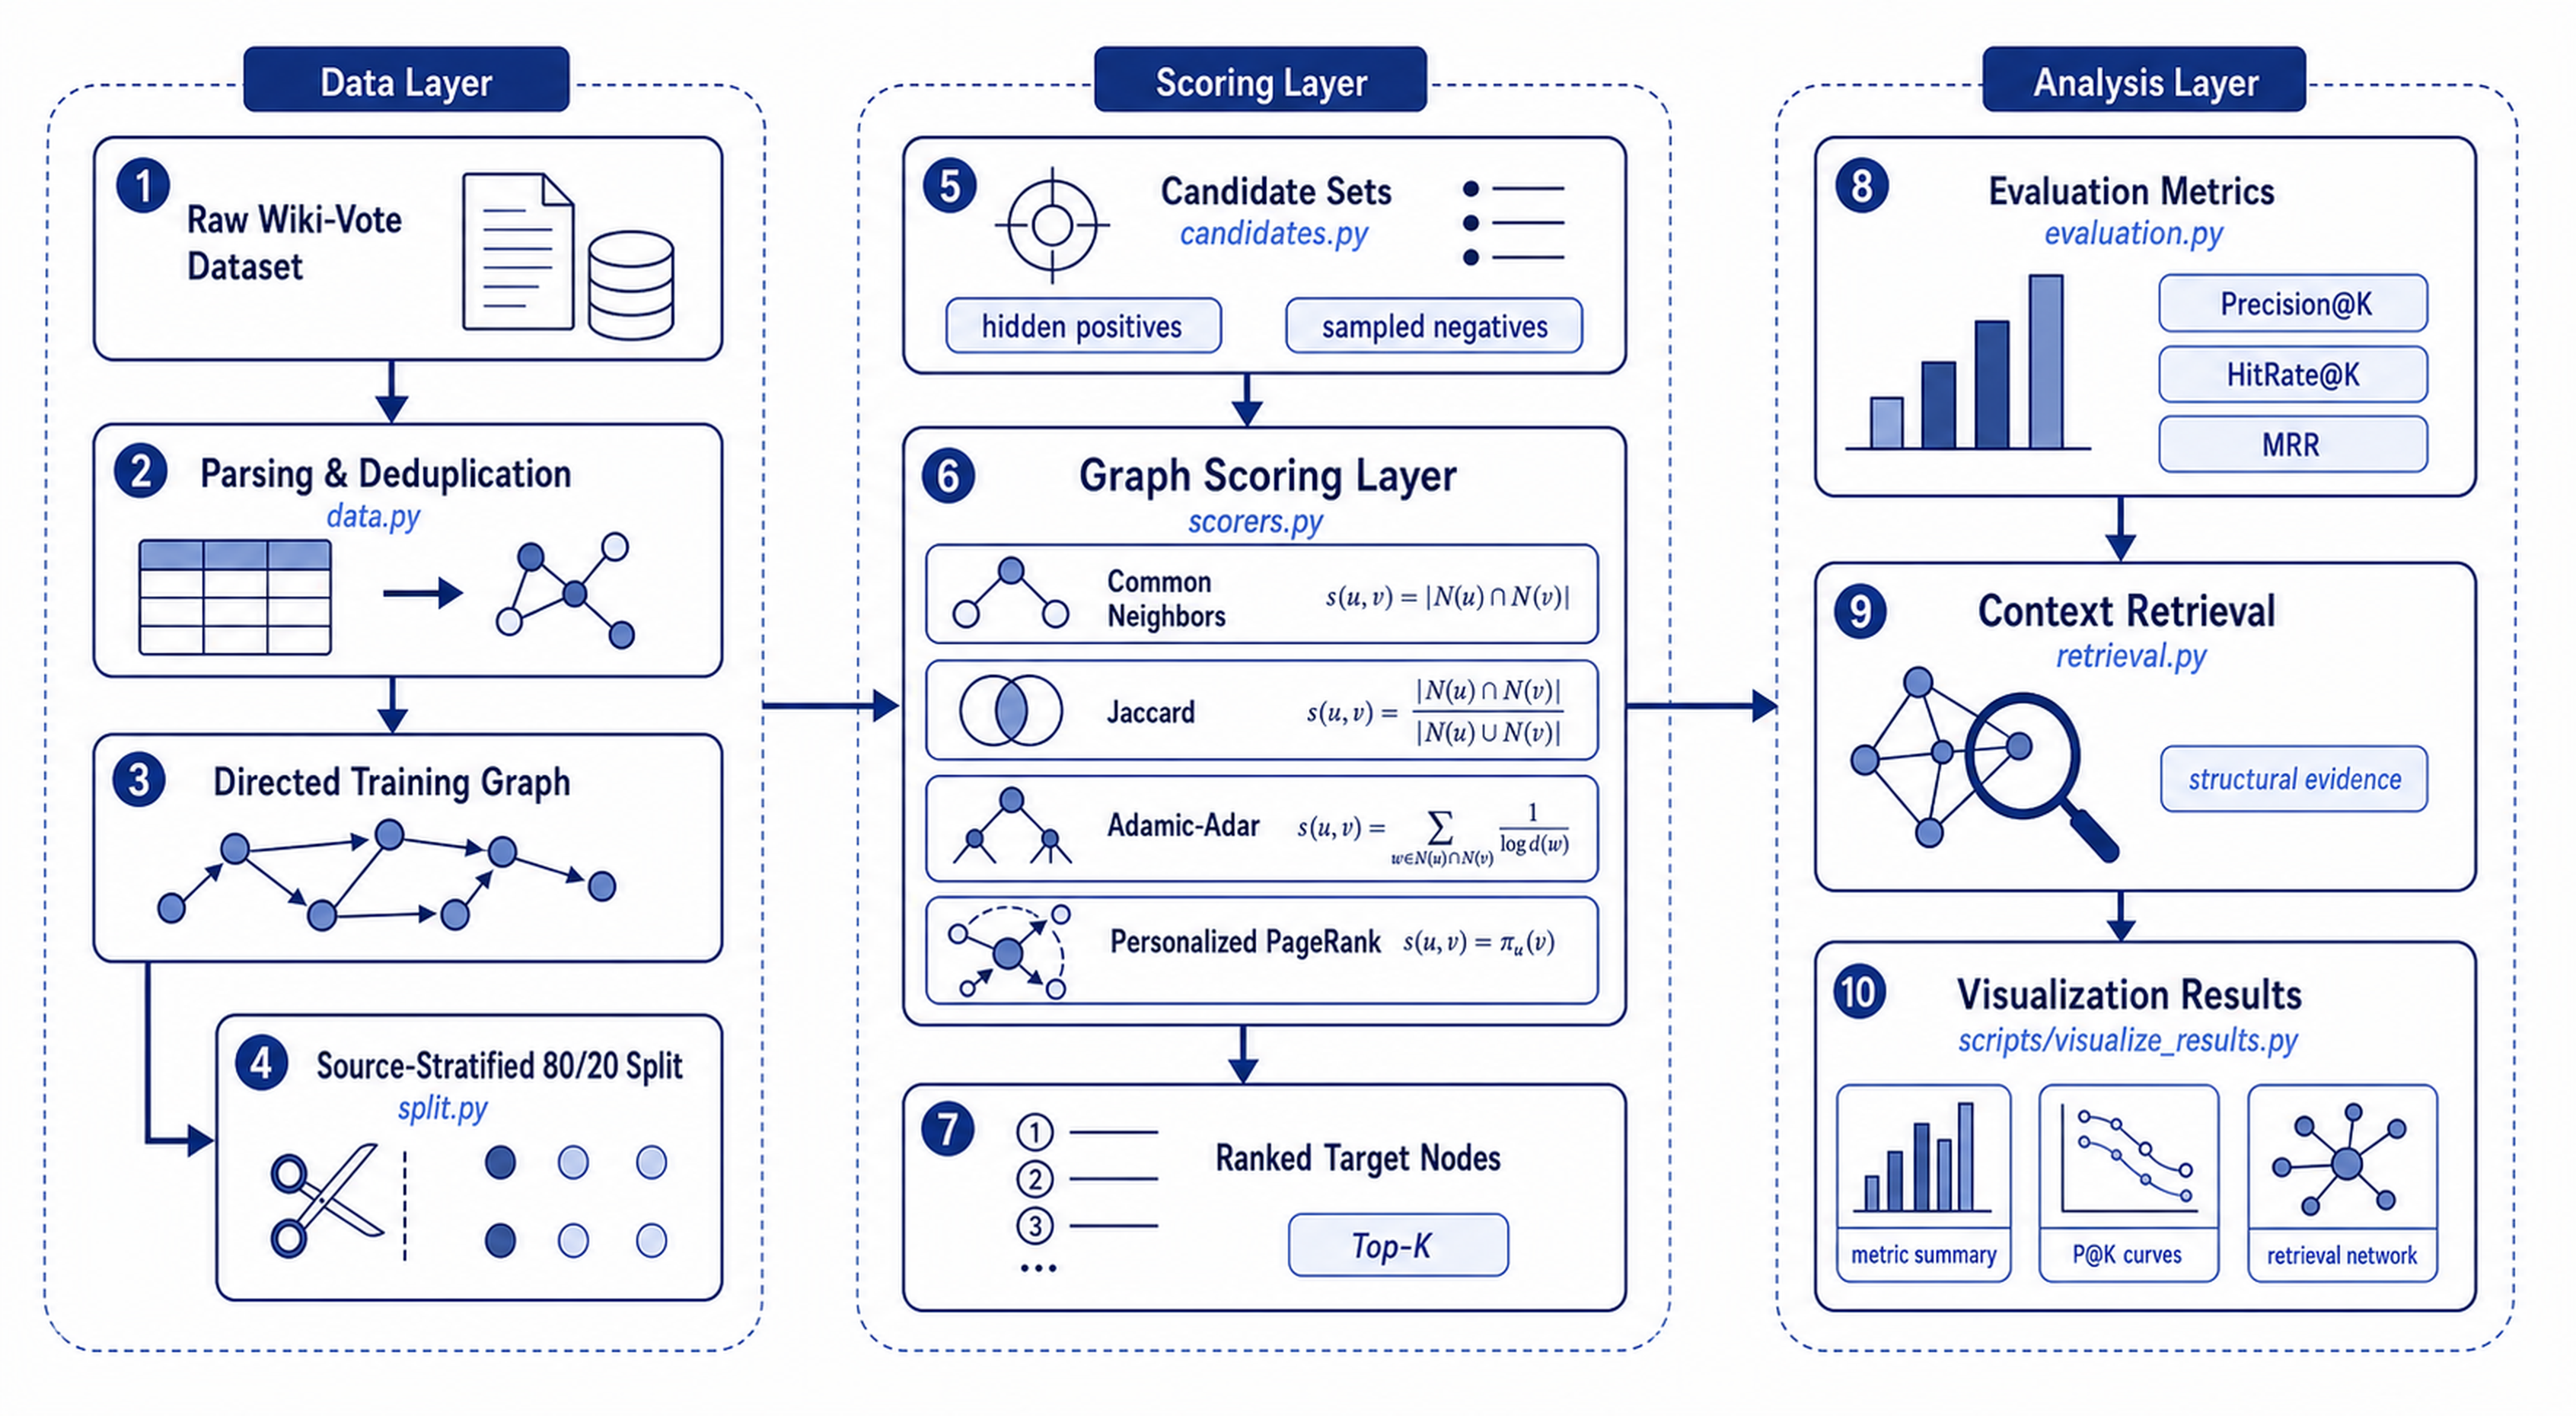
\includegraphics[width=0.93\textwidth,height=0.42\textheight,keepaspectratio]{figures/pipeline_workflow_300dpi.png}
\caption{Implemented Net RAG workflow. The repository separates the system into a data layer, a graph scoring layer, and an analysis layer, allowing retrieval quality to be measured before integration with a downstream language generator.}
\label{fig:pipeline}
\end{figure*}

\section{Related Work}
Retrieval has long been a central mechanism for grounding natural language systems. Classical sparse retrieval methods such as BM25 are rooted in probabilistic relevance modeling and remain strong baselines for document search \citep{robertson2009bm25}. Dense passage retrieval later showed that dual-encoder representations can retrieve semantically related passages even when exact lexical overlap is weak \citep{karpukhin2020dpr}. RAG combines this retrieval step with a parametric generator, allowing language models to condition generation on external non-parametric memory \citep{lewis2020rag}. This design is especially relevant for domains where model parameters alone cannot guarantee factuality, freshness, or coverage.

GraphRAG extends retrieval beyond independent text chunks. Instead of treating candidate contexts as isolated documents, graph-based retrieval models organize entities, documents, and relations into a structured index. This enables systems to retrieve context through relational paths, community structure, or global summaries rather than only through vector similarity. Recent GraphRAG work demonstrates that graph indexes can support query-focused summarization over large collections by combining local evidence with global community-level context \citep{edge2024graphrag}. The present project follows the same motivation but narrows the research question to the retrieval module: can graph structure alone recover hidden relevant nodes?

The task is also connected to classical link prediction. Liben-Nowell and Kleinberg formalized link prediction as inferring missing or future social interactions from a network snapshot and showed that graph proximity features can be predictive \citep{liben2007link}. Common Neighbors and Jaccard are local neighborhood-overlap heuristics; Adamic-Adar refines overlap by assigning more value to rare shared neighbors \citep{adamic2003friends}. PageRank and Personalized PageRank provide random-walk views of node importance and source-conditioned relevance \citep{page1999pagerank,jeh2003scaling}. These methods are attractive for a compact GraphRAG retrieval module because they are interpretable, deterministic under fixed seeds, and do not require task-specific neural training.

A parallel line of graph representation learning learns continuous node embeddings from random walks or biased neighborhood sampling. DeepWalk generalizes language-model-style sequence learning to graph walks \citep{perozzi2014deepwalk}, while node2vec introduces biased random walks to balance local and structural neighborhoods \citep{grover2016node2vec}. Such embedding approaches can be powerful for downstream prediction, but they introduce additional training objectives and hyperparameters. This project instead emphasizes transparent graph scorers, which makes the retrieval behavior easier to audit in a small course-scale GraphRAG pipeline.

The experimental dataset comes from SNAP's Wikipedia Vote Network, whose source material is associated with work on signed social networks and link prediction in online communities \citep{leskovec2010signed,leskovec2010predicting,snapnets}. The implementation uses NetworkX for graph construction and traversal \citep{hagberg2008networkx}.

\section{Methodology}
\subsection{Problem Formulation}
Figure~\ref{fig:pipeline} summarizes the implemented workflow. Let $G=(V,E)$ be the directed Wiki-Vote graph. The project hides a subset of edges $E_{\mathrm{test}}$ and builds a training graph $G_{\mathrm{train}}=(V,E_{\mathrm{train}})$. For a source node $s$, the retrieval module ranks candidate targets $t$ that are not already visible as training outgoing edges from $s$. Hidden test edges are positive candidates, and randomly sampled non-existent edges are negative candidates.

The output is a ranked list:
\[
R_s = \operatorname{rank}_{t \in C_s} f(s,t),
\]
where $C_s$ is the candidate set for source $s$ and $f$ is a graph scoring function.

\subsection{Data Preparation}
The raw file \texttt{Wiki-Vote.txt} is parsed directly. Comment lines are skipped, edge rows are converted into integer node pairs, and duplicate edges are removed. Because the dataset does not include timestamps for each edge in the local task file, the project uses a deterministic random split. For each source node with at least two outgoing edges, approximately $20\%$ of its targets are sampled into the test set, while at least one outgoing edge is kept for training. Sources with one outgoing edge remain in the training graph.

SNAP reports 7,115 nodes and 103,689 edges for the Wiki-Vote network \citep{snapnets}. The repository's default split with seed 42 produces 82,822 training edges and 20,867 testing edges from 103,689 unique edges.

\subsection{Graph Scoring Functions}
The project evaluates four scoring functions. Common Neighbors counts neighbor overlap in an undirected projection:
\[
f_{\mathrm{CN}}(s,t)=|\Gamma(s)\cap\Gamma(t)|.
\]
The Jaccard coefficient normalizes overlap by the union size:
\[
f_{\mathrm{Jaccard}}(s,t)=
\frac{|\Gamma(s)\cap\Gamma(t)|}{|\Gamma(s)\cup\Gamma(t)|}.
\]
Adamic-Adar discounts high-degree common neighbors:
\[
f_{\mathrm{AA}}(s,t)=
\sum_{z\in \Gamma(s)\cap\Gamma(t)}\frac{1}{\log |\Gamma(z)|}.
\]
These three scorers use the undirected training projection to reduce sparsity.

Personalized PageRank is implemented as an approximate random-walk scorer on the directed training graph. For each source node, the implementation simulates source-centered walks with restart probability 0.15, 400 walks, and walk length 20. Candidate targets are scored by normalized visit frequency. This produces a practical approximation to source-conditioned graph relevance.

\subsection{Candidate Sampling and Evaluation}
For every source node with hidden positives, the candidate set includes its true hidden targets and up to 100 randomly sampled negative targets that are not edges in the full graph. The random sampler is deterministic under the configured seed.

The ranking is evaluated with Macro Precision@K, HitRate@K, and mean reciprocal rank (MRR). Precision@K measures the average fraction of top-$K$ candidates that are true hidden edges. HitRate@K records whether at least one hidden edge appears in the top-$K$ list. MRR rewards algorithms that place the first positive target early in the ranking.

\section{Experiments}
The experiments use the repository defaults: seed 42, test ratio 0.2, $K=10$, and 100 negative samples per source. The full pipeline is executed from the repository root in four stages:
\begin{enumerate}
    \item prepare the train/test edge split from \texttt{Wiki-Vote.txt};
    \item evaluate all graph scorers over sampled candidate sets;
    \item retrieve the top related nodes for a selected source user;
    \item generate summary plots from saved metrics and ranking files.
\end{enumerate}

The experiments were conducted on a Python 3.12 workstation equipped with an NVIDIA GeForce RTX 4080 GPU. The software stack uses NetworkX as the graph computation framework for graph construction, neighborhood traversal, and random-walk-based retrieval. NumPy and pandas are used for deterministic candidate processing and metric aggregation, while matplotlib is used to generate the visual analysis figures. The experimental artifacts are written as CSV, JSON, and PNG files so that each stage can be inspected and reproduced independently.

The split protocol is source-node stratified so that evaluated sources retain visible outgoing graph context in the training graph. This design is important for retrieval: if all outgoing edges of a low-degree source were hidden, neighborhood-based methods would have no local evidence from which to rank targets. Candidate construction combines all hidden positives for each evaluated source with a fixed-size random negative set. The negative edges are sampled from node pairs that do not appear in the full graph, which gives each scorer a controlled ranking problem while avoiding the infeasible cost of scoring all possible non-edges.

The implementation is intentionally modular: it evaluates the retrieval component of a GraphRAG pipeline before connecting it to a full LLM answering system. This separation makes retrieval behavior measurable without confounding it with generator quality, prompt design, or answer evaluation. In the current configuration, the most expensive component is approximate Personalized PageRank random-walk scoring over the directed training graph.

\section{Results}
Table~\ref{tab:main-results} reports the saved full-dataset retrieval results. Personalized PageRank is the strongest scorer on all three metrics. Compared with Adamic-Adar, the best local-overlap baseline, Personalized PageRank improves Precision@10 by 0.008825, HitRate@10 by 0.077789, and MRR by 0.048910. The largest gain appears in HitRate@10, indicating that source-conditioned random walks are particularly effective at bringing at least one hidden positive edge into the top retrieved context set.

\begin{table}[t]
\centering
\caption{Full-dataset retrieval performance with $K=10$ and 100 negative candidates per source.}
\label{tab:main-results}
\scriptsize
\begin{tabular}{@{}lccc@{}}
\toprule
Algorithm & P@10 & HR@10 & MRR \\
\midrule
Common Neighbors & 0.229641 & 0.711373 & 0.493400 \\
Jaccard & 0.219742 & 0.698766 & 0.420111 \\
Adamic-Adar & 0.230472 & 0.714056 & 0.502139 \\
Personalized PR & \textbf{0.239297} & \textbf{0.791845} & \textbf{0.551049} \\
\bottomrule
\end{tabular}
\end{table}

\begin{figure}[t]
\centering
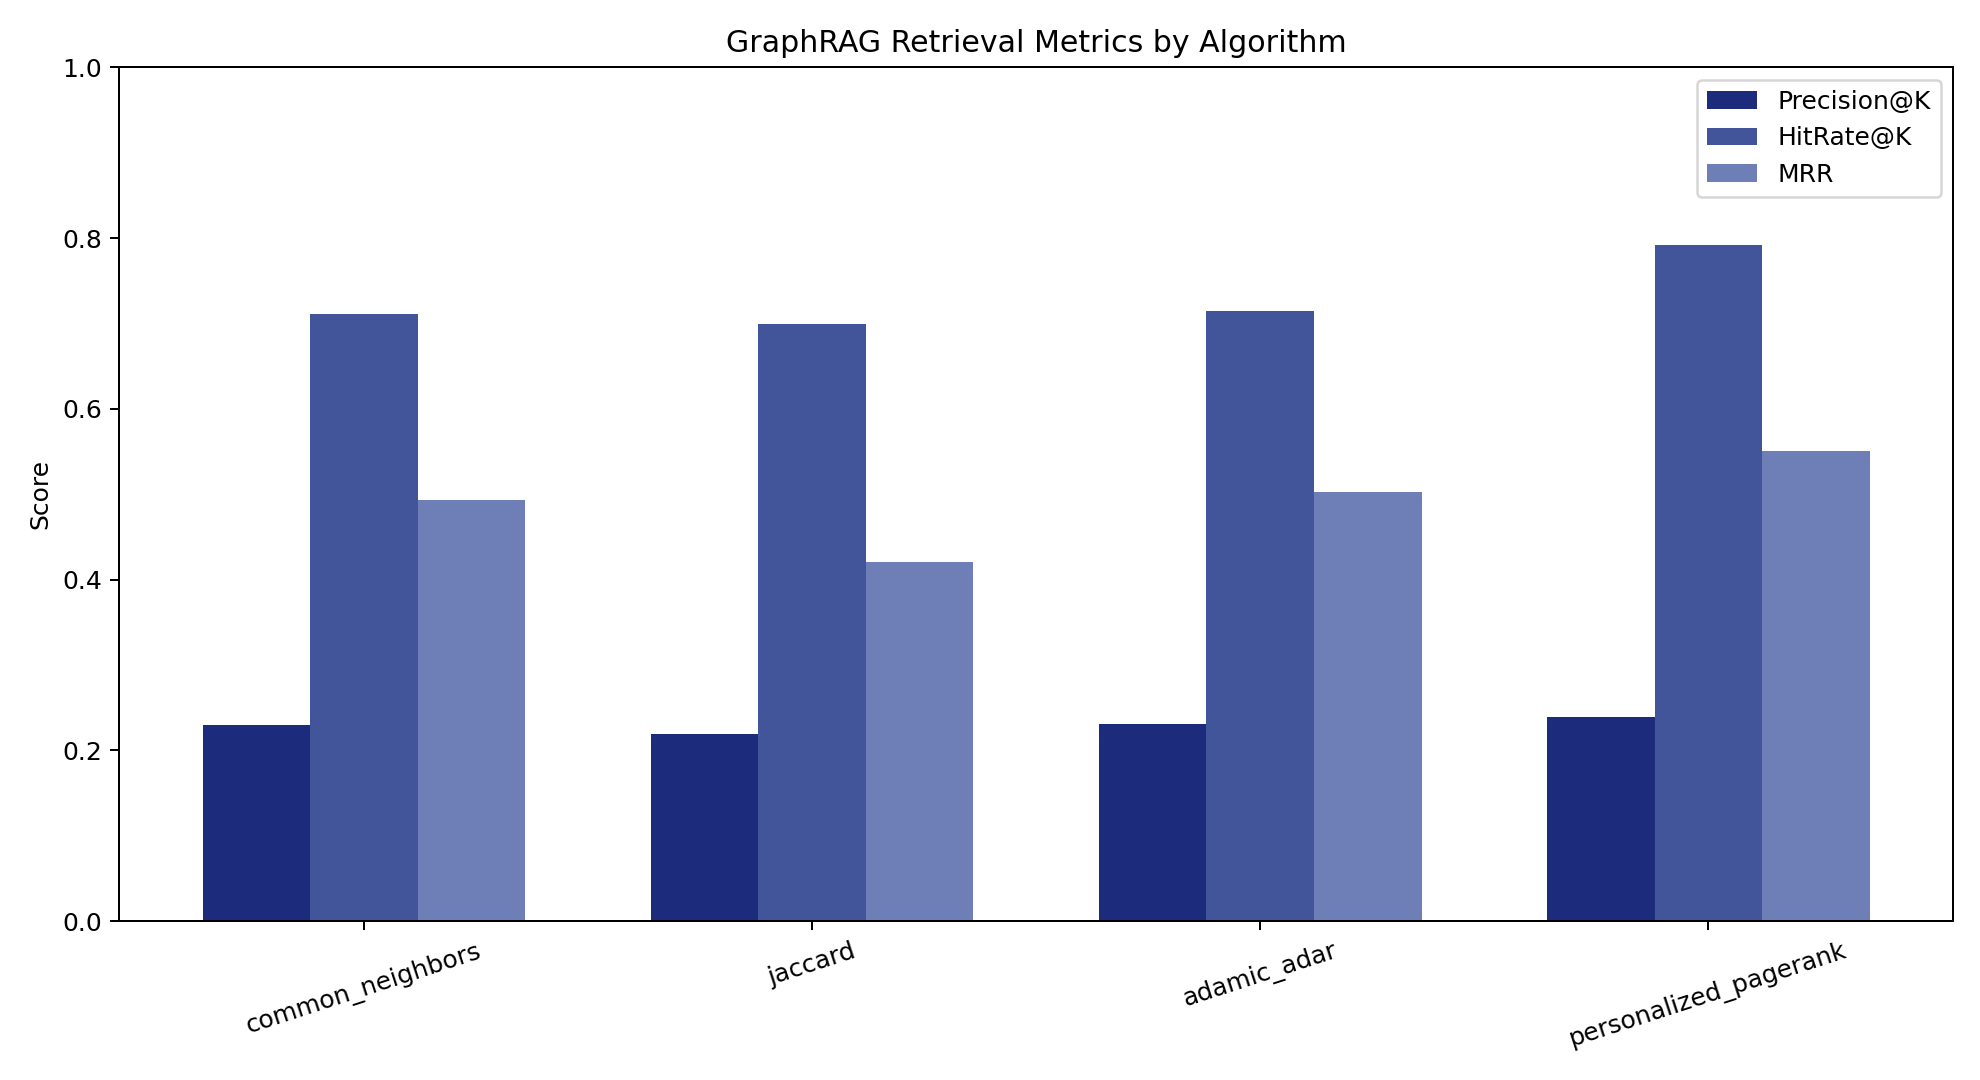
\includegraphics[width=\linewidth]{figures/metrics_summary.png}
\caption{Metric summary across graph retrieval algorithms.}
\label{fig:metrics-summary}
\end{figure}

\begin{figure}[t]
\centering
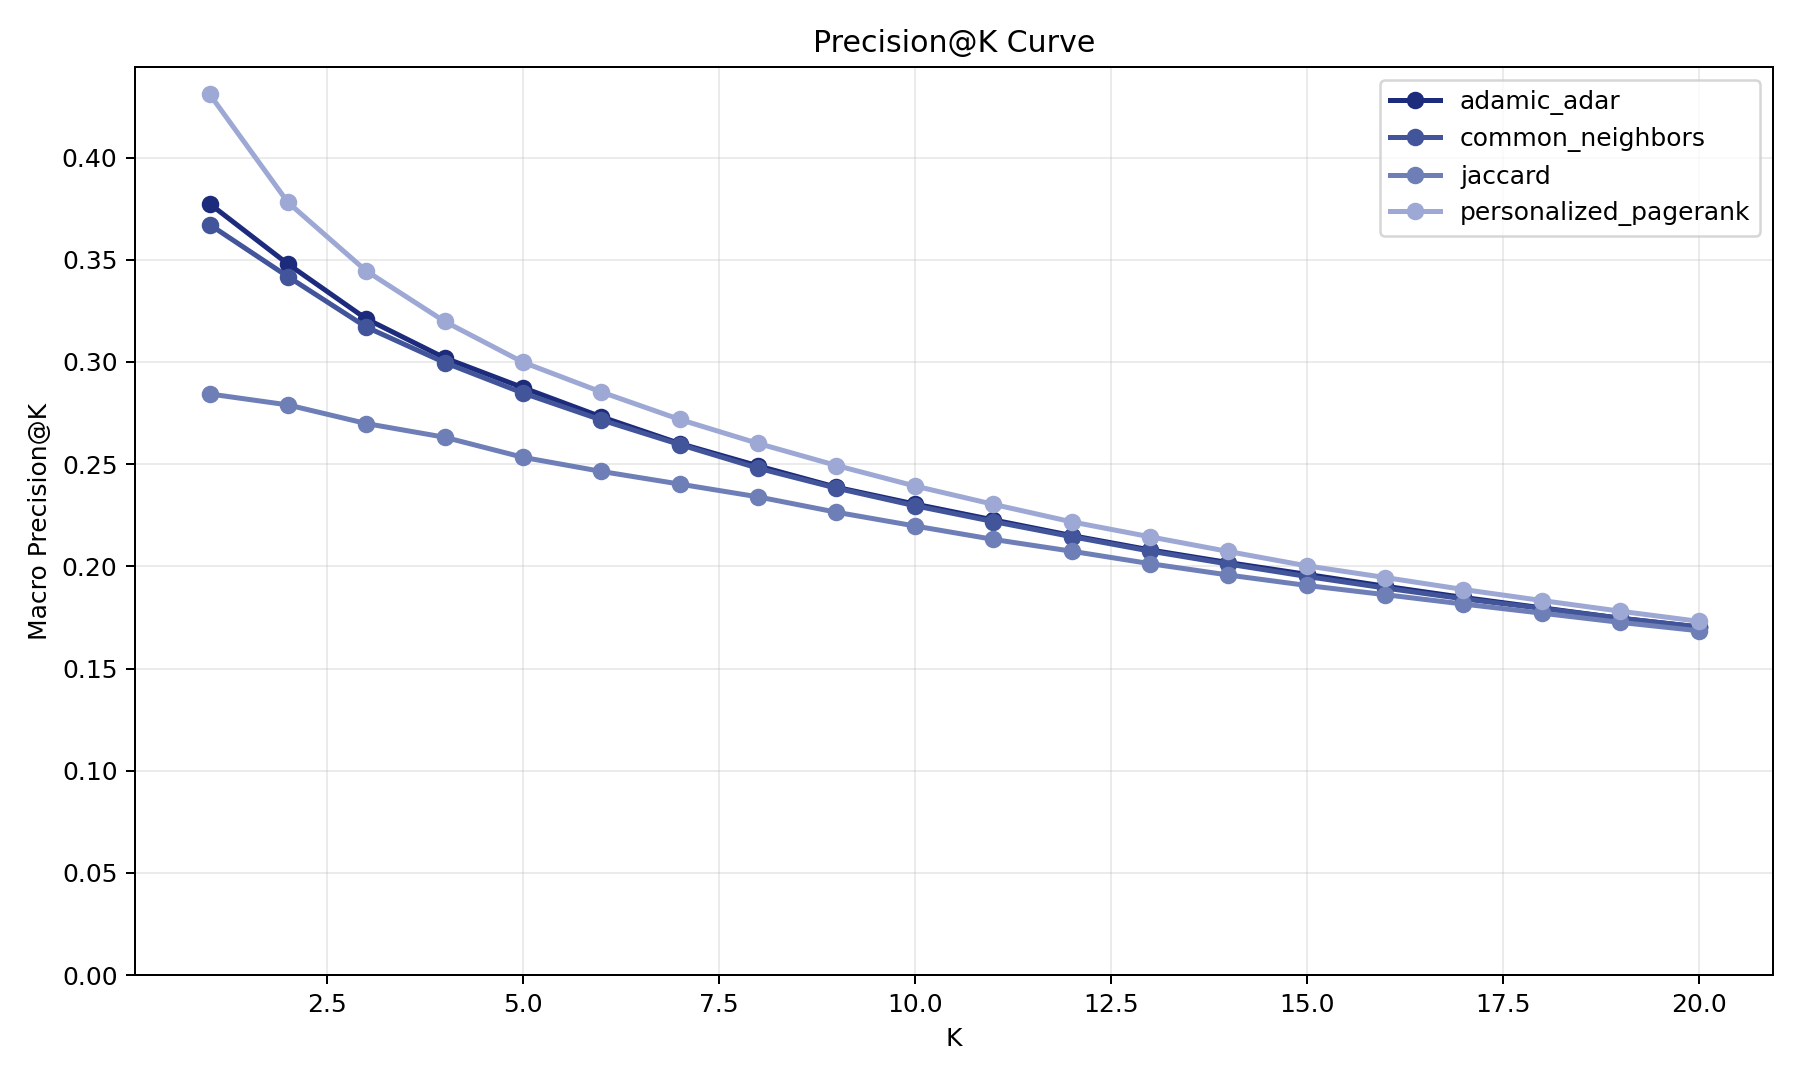
\includegraphics[width=\linewidth]{figures/precision_at_k_curve.png}
\caption{Precision@K curve showing how retrieval quality changes as $K$ increases.}
\label{fig:precision-curve}
\end{figure}

Figure~\ref{fig:metrics-summary} confirms that Personalized PageRank dominates the aggregate metrics, while Figure~\ref{fig:precision-curve} shows that the ranking behavior remains competitive beyond the single $K=10$ operating point. This matters for GraphRAG because a downstream generator may consume different context budgets depending on prompt length, model context window, and latency constraints. A scorer that remains stable across cutoffs is easier to deploy than one that only performs well at a narrowly tuned $K$.

\begin{figure}[t]
\centering
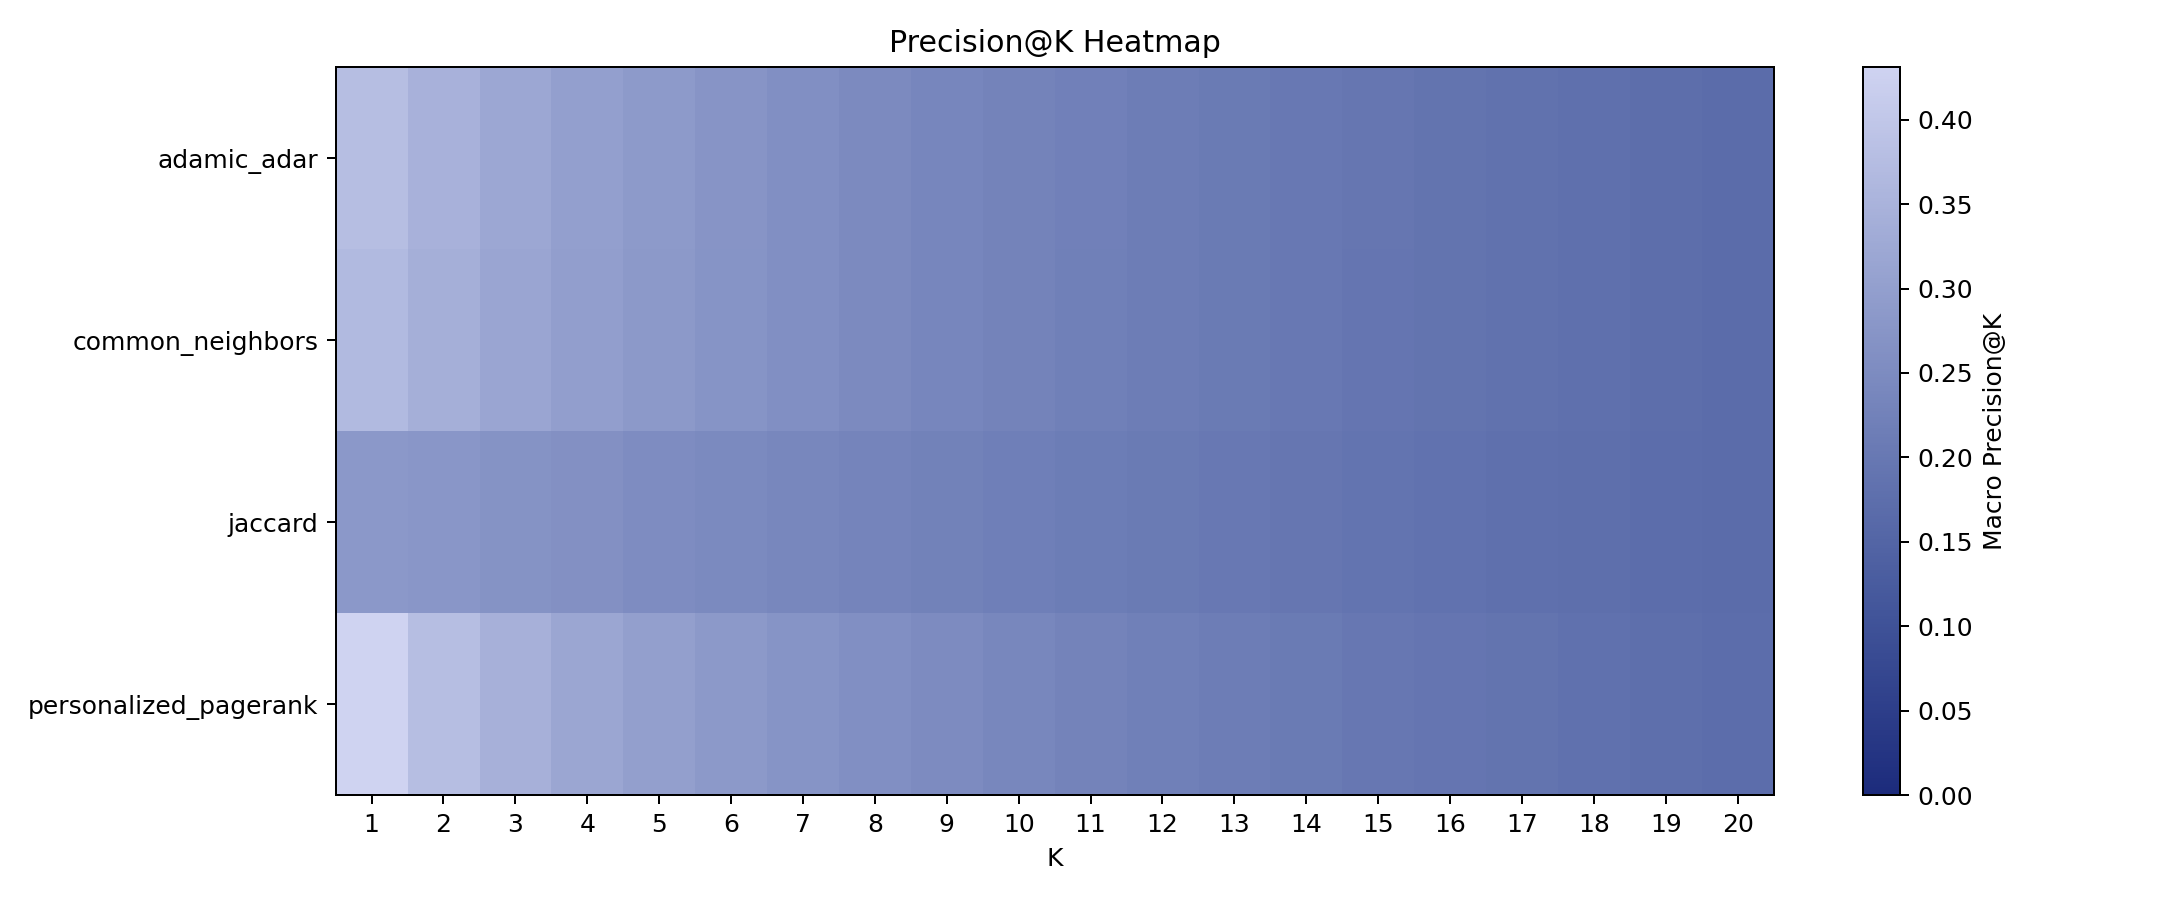
\includegraphics[width=\linewidth]{figures/precision_at_k_heatmap.png}
\caption{Precision@K heatmap for comparing algorithms and cutoff values.}
\label{fig:heatmap}
\end{figure}

\begin{figure}[t]
\centering
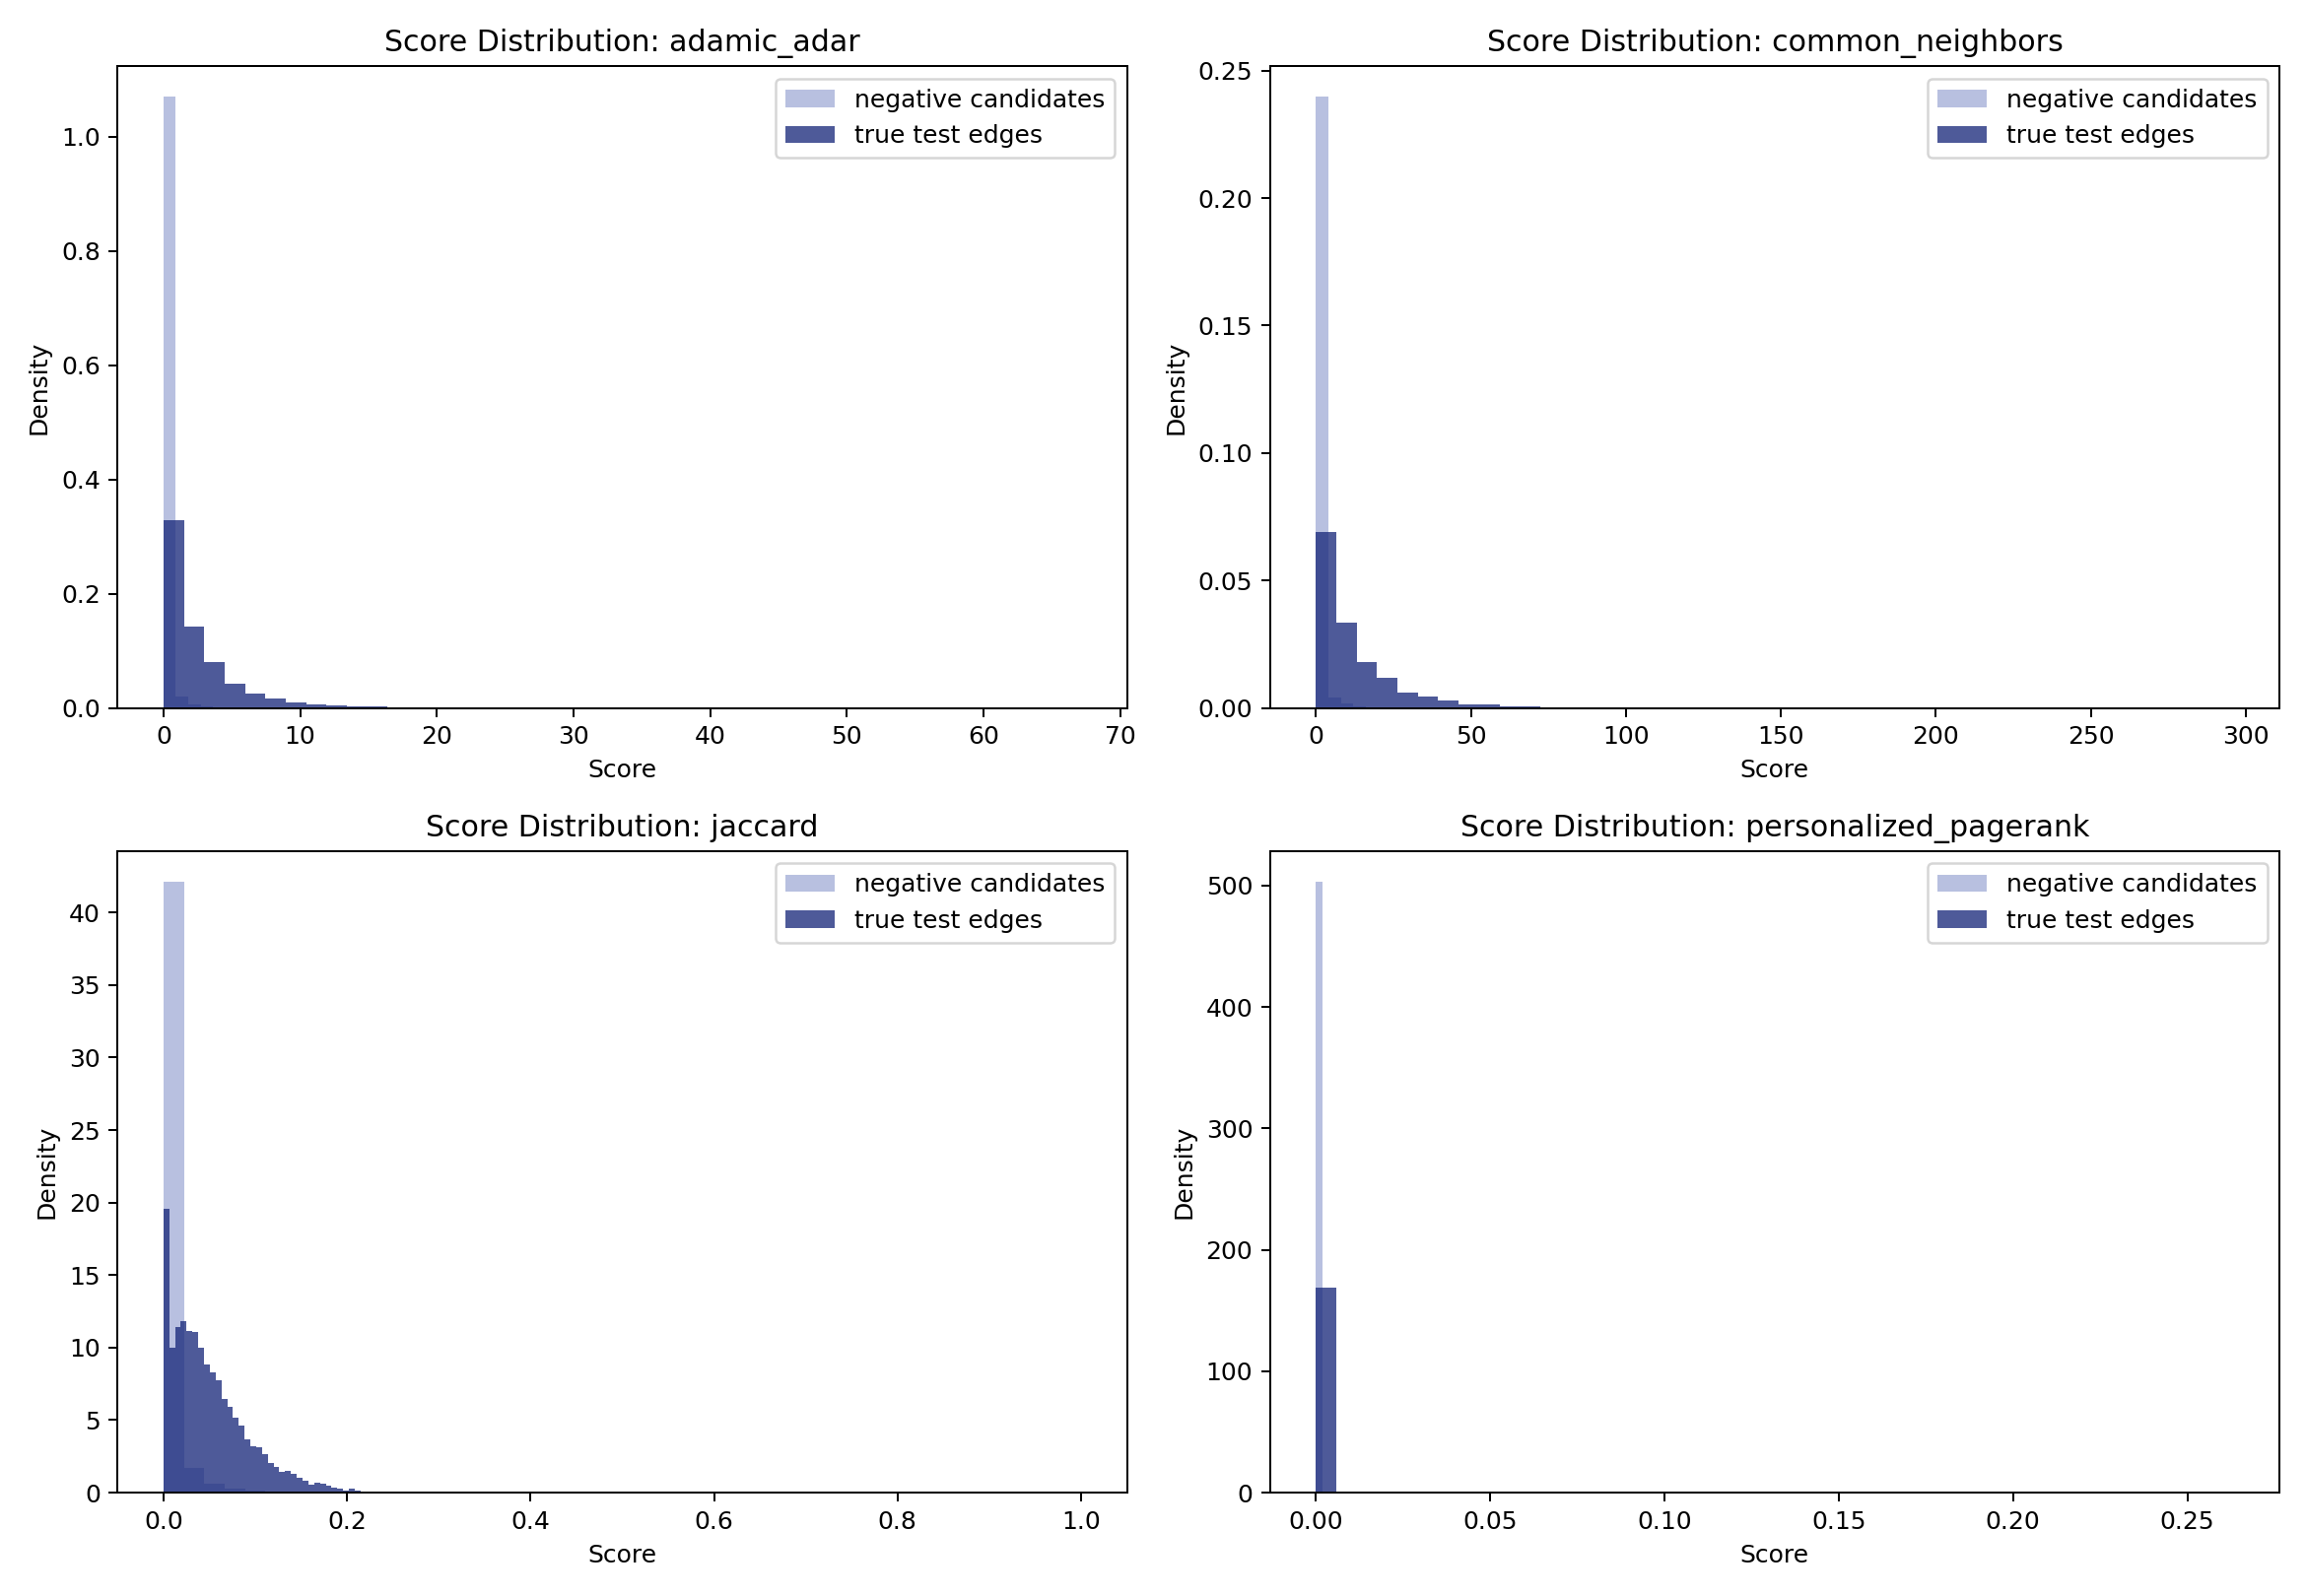
\includegraphics[width=\linewidth]{figures/score_distribution_positive_negative.png}
\caption{Score distribution for positive hidden edges and sampled negative candidates.}
\label{fig:score-dist}
\end{figure}

Figures~\ref{fig:heatmap} and~\ref{fig:score-dist} provide a more diagnostic view of ranking quality. The heatmap makes the cutoff sensitivity visible and shows that methods based on richer structural evidence are less fragile as the allowed retrieval set changes. The score distribution further explains the numerical results: successful retrieval requires not only high scores for positives, but also sufficient separation from sampled negatives. Personalized PageRank benefits from multi-hop directed evidence, whereas local overlap methods can assign similar low scores when two candidate nodes share few immediate neighbors.

\begin{figure}[t]
\centering
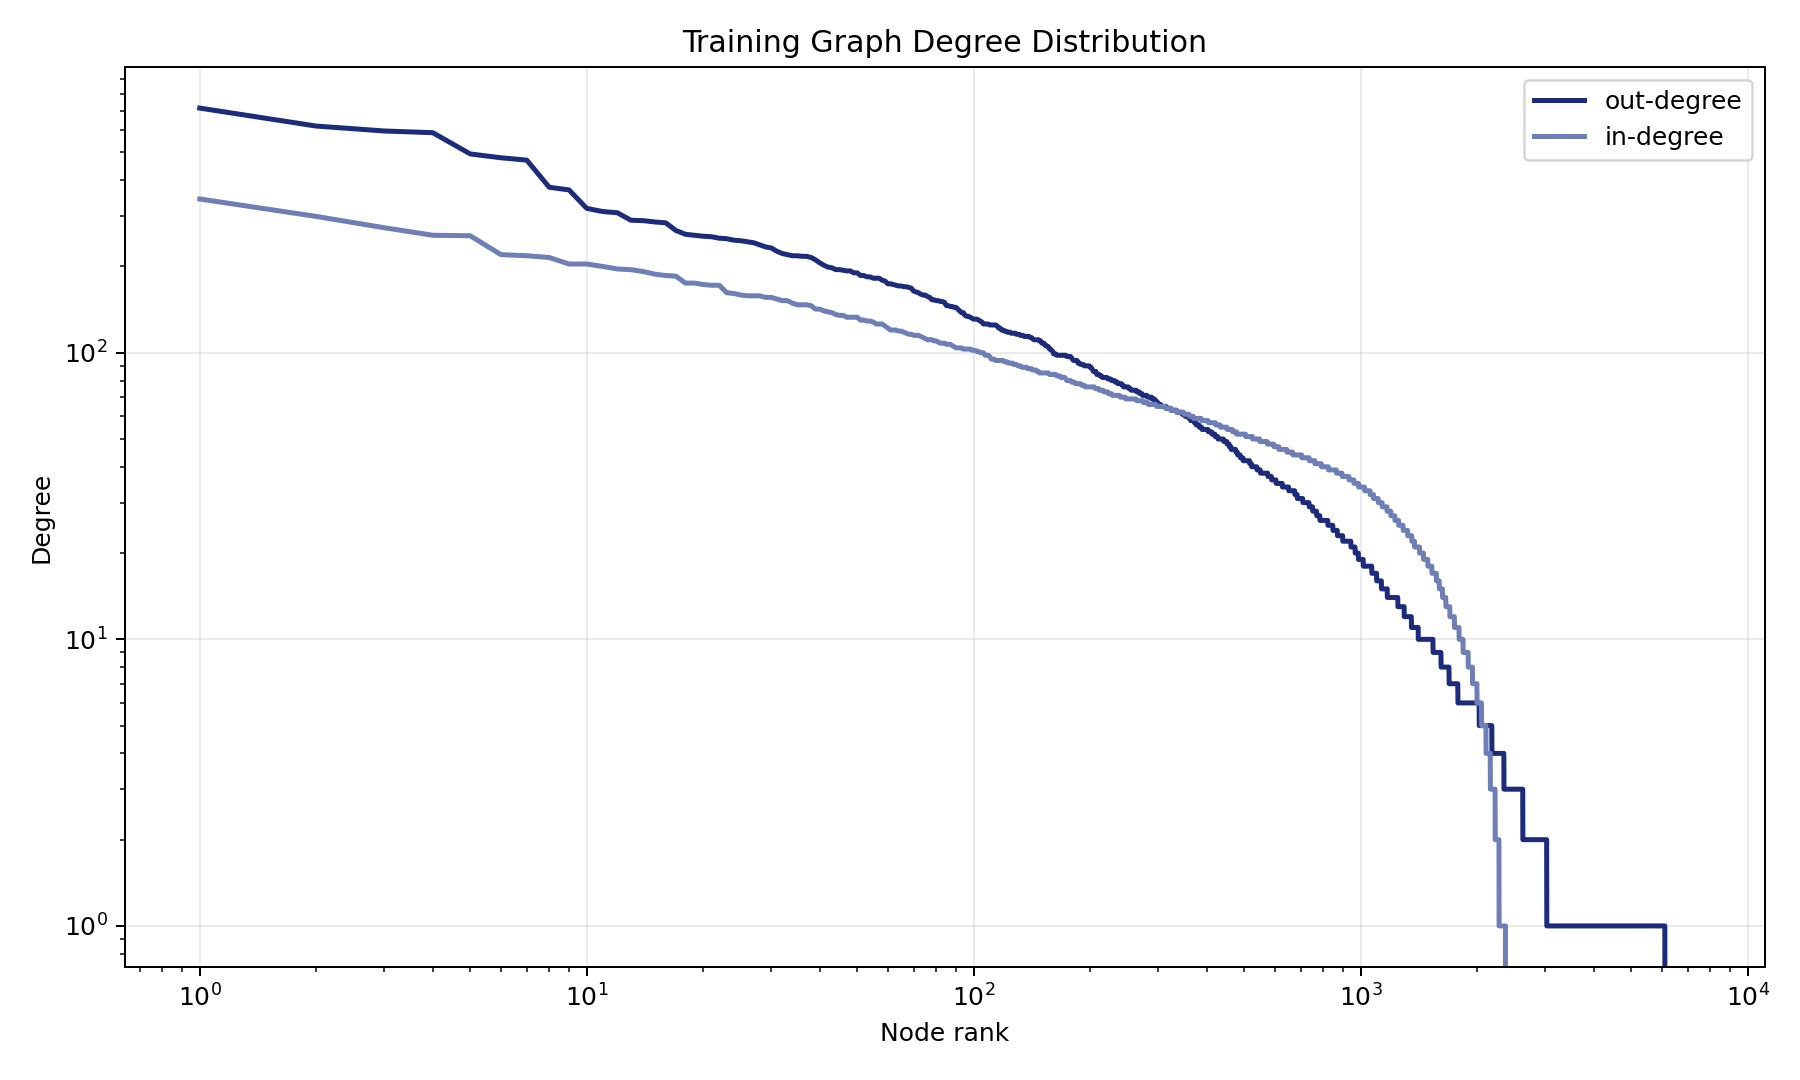
\includegraphics[width=\linewidth]{figures/train_degree_distribution.png}
\caption{Training graph degree distribution, showing the heavy-tailed structure typical of real social networks.}
\label{fig:degree}
\end{figure}

\begin{figure}[t]
\centering
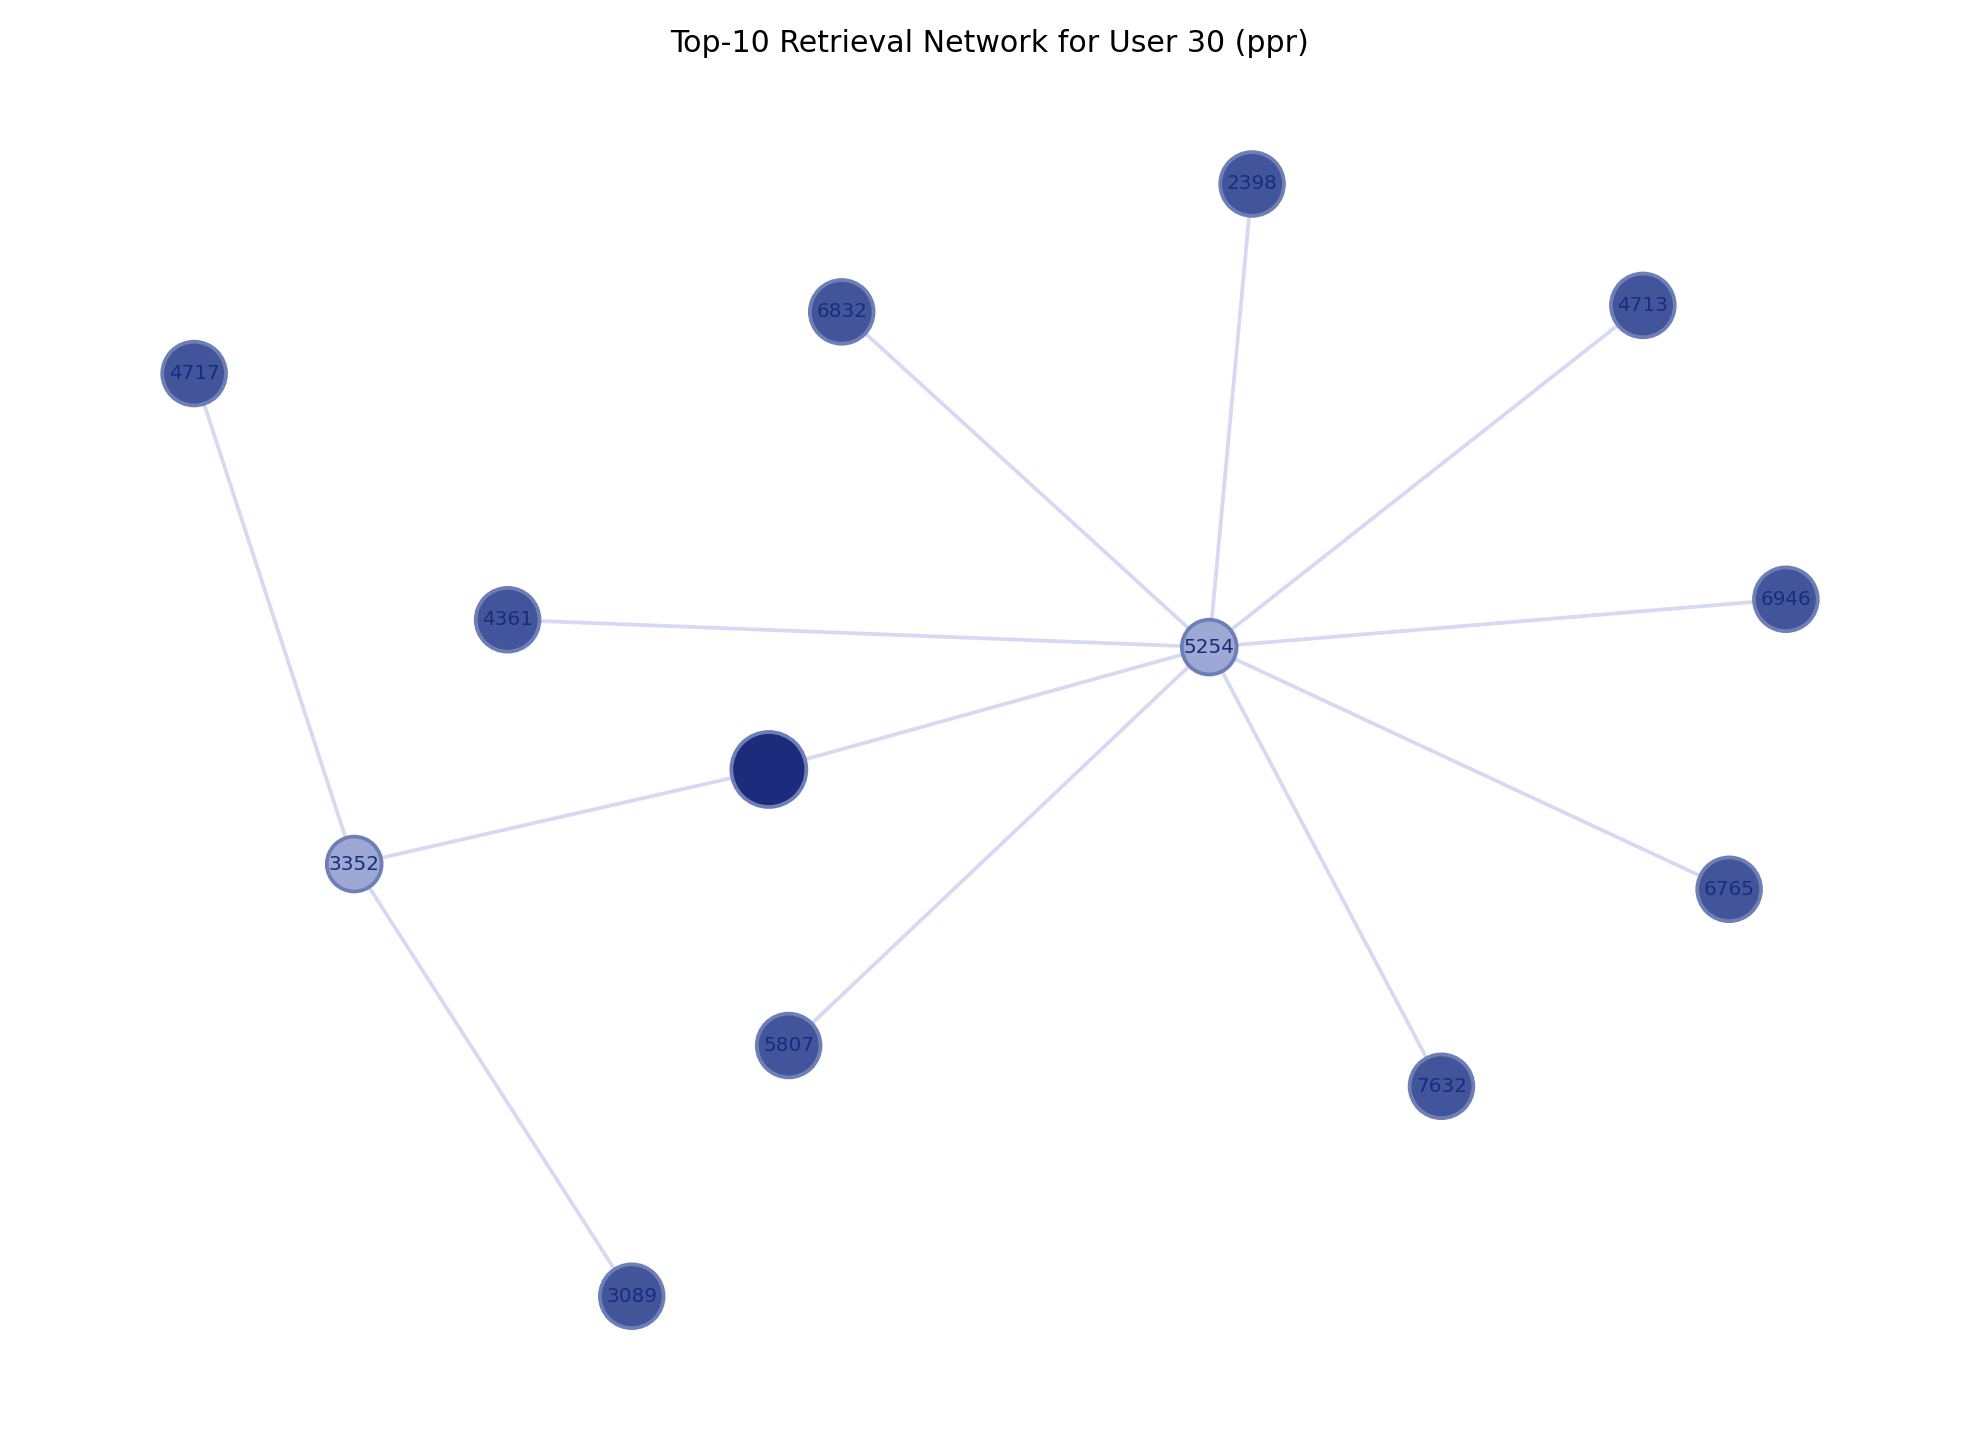
\includegraphics[width=\linewidth]{figures/user_30_ppr_retrieval_network.png}
\caption{Example Personalized PageRank retrieval network for user 30.}
\label{fig:retrieval-network}
\end{figure}

Figures~\ref{fig:degree} and~\ref{fig:retrieval-network} connect the quantitative metrics back to graph structure. The degree distribution shows a highly skewed training graph, which is expected in social and voting networks. This skew explains why Jaccard underperforms: normalizing by the union of neighborhoods can penalize candidates connected through high-degree regions, even when those regions are informative. Common Neighbors and Adamic-Adar perform better because they preserve direct overlap signals, but they remain local. The retrieval network example shows the practical value of the repository's \texttt{retrieval.py} module: the output is not just a score table, but a ranked context set with structural evidence such as shared neighbors or short graph paths.

Overall, the experimental results support three observations. First, graph-only retrieval is feasible on the full Wiki-Vote network without neural training. Second, local graph heuristics provide strong and interpretable baselines, but their effectiveness is constrained by sparse immediate neighborhoods. Third, approximate Personalized PageRank is the best fit for this repository because it preserves directionality, uses multi-hop evidence, and produces the strongest ranking metrics under the same candidate sampling protocol.

\clearpage

\section{Conclusion}
This project demonstrates a reproducible GraphRAG retrieval module by turning context retrieval into link prediction on the Wiki-Vote graph. The results show that approximate Personalized PageRank provides the best retrieval quality among the implemented scorers, outperforming local overlap methods on Precision@10, HitRate@10, and MRR. More broadly, the study supports the value of graph-aware retrieval when relevant context is relational rather than purely textual.

The main limitation is that the system stops at retrieval: it does not yet feed retrieved graph context into an LLM, evaluate generated answers, or compare against dense text retrieval. Future work should add textual node attributes, test graph-plus-vector hybrid retrieval, and measure the downstream effect of retrieved graph context on answer factuality and citation quality.

\bibliographystyle{plainnat}
\bibliography{references}

\end{document}
